\documentclass{beamer}
\mode<presentation> {
\usetheme{Berlin}

\setbeamertemplate{footline}[page number] 
\setbeamertemplate{navigation symbols}{} 
\setbeamertemplate{itemize item}[square]
\setbeamertemplate{itemize subitem}[circle]
\setbeamertemplate{itemize subsubitem}[default]
}
\usepackage{graphicx}
\usepackage{minted}
\usepackage{setspace}
\setlength{\columnsep}{1cm}

\newenvironment{mysubsec}[1]
{   \begin{frame}
	\frametitle{#1} }
{ \end{frame} }

%----------------------------------------------------------------------------------------
%   TITLE PAGE
%----------------------------------------------------------------------------------------
\title{Towards a Dataflow Approach to \\ Robot Programming}
\author{Orestis Melkonian} 
\institute[UoA] {
	Software \& Knowledge Engineering Laboratory (SKEL)\\
	\medskip
	\textit{NCSR "Demokritos"}
}
\date{}
\begin{document}
\begin{frame} \titlepage \end{frame}

\begin{frame} \frametitle{Overview} \tableofcontents \end{frame}
%----------------------------------------------------------------------------------------
\section{Motivation}
	\begin{frame}[allowframebreaks] \frametitle{Motivation}		
		\begin{itemize}
		\item \textbf{Common Patterns}
			\begin{itemize}
			\item Robot perception architecture
			\item Feedback loop controllers			
			\end{itemize}
			\medskip
			\center 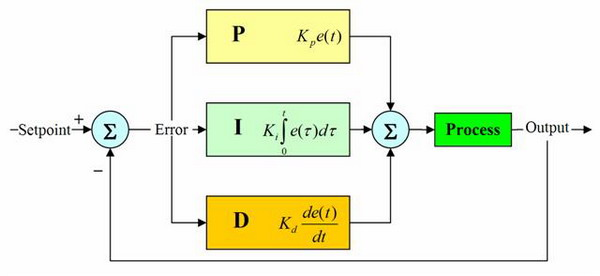
\includegraphics[scale=0.4,keepaspectratio]{pics/pid.jpg}						
		\end{itemize}
		\framebreak		
		\begin{itemize}
		\item \textbf{ROS}: Robot Operating System
			\begin{itemize}
			\item Hardware abstraction
			\item Reusability
			\item Language-agnostic open-source middleware
			\item Publish-Subscribe design pattern
			\item Communication via "topics"
			\item Status Quo
				\begin{itemize}
				\item Almost all code written in C++ and Python
				\item Callbacks			
				\item Dataflow nature so far ignored
				\end{itemize}					
			\end{itemize}
		\end{itemize}		
	\end{frame}
%------------------------------------------------------------------
\section{Stream Framework}
	\begin{frame} \frametitle{Stream Framework}
		\begin{itemize}		
		\item Topics as streams
		\item At a micro-level, replace callback "internal plumbing" with clean functional declarations
		\item At a macro-level, acts as a coordinating language adding to the composability of ROS
		\item \textbf{Extensibility}
			\begin{itemize}
			\item Strategy design pattern for evaluation
			\item Coder simply declares a dataflow graph
			\end{itemize}
		\item \textbf{Advantages}
			\begin{itemize}						
			\item Decouple design (what to do) from execution (how to do it)
			\item Cleaner, easier to maintain code
			\item Implicit concurrency
			\item Implicit message-passing
			\end{itemize}
		\end{itemize}
	\end{frame}	
%------------------------------------------------------------------
\section{Future Work}
	\begin{mysubsec}{Future Work: Optimization}
		\begin{itemize}
		\item General graph transformations
			\begin{itemize}
			\item Apply some simple heuristics
			\item Preserve semantics
			\item Back-ends continue with more specific optimizations
			\end{itemize}
		\item Network-aware placement
			\begin{itemize}
			\item Fusion/fission to reach desired granularity
			\item Dynamic reconfiguration
			\end{itemize}
		\end{itemize}
	\end{mysubsec}
	\begin{mysubsec}{Future Work: DSL}		
		\begin{itemize}
		\item Minimize boilerplate code
		\item More intuitive syntax
		\item Embedded in Scala
			\begin{itemize}
			\item Functional
			\item Inherit rich type system
			\item Little programming effort
			\end{itemize}
		\item Restrict host language
			\begin{itemize}
			\item Single-assignment
			\item Restricted resource usage
			\end{itemize}
		\item Impose a specific program structure 
			\begin{itemize} \item Minimize design flaws \end{itemize}
		\end{itemize}
	\end{mysubsec}
%------------------------------------------------------------------
\section{Demos}
	\begin{mysubsec}{Demos: Hamming Numbers ($ 2^i 3^j 5^k $)}
	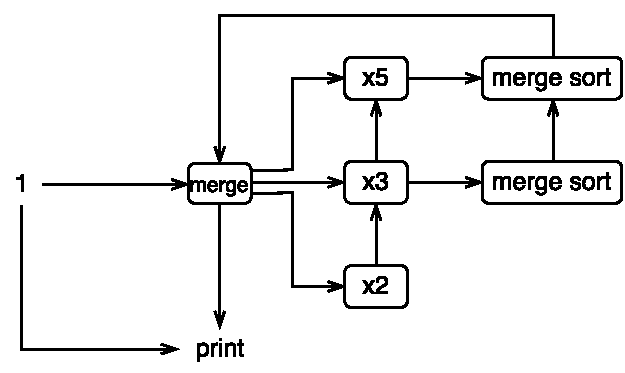
\includegraphics[scale=0.8,keepaspectratio]{pics/Hamming.pdf}
	\end{mysubsec}
%------------------------------------------------------------------	
\begin{frame}
	\Huge{\centerline{The End}}
\end{frame}
%------------------------------------------------------------------
\end{document}
